% Remove the \emph on ``transparently'' and ``while'' again.  Pantazis, I'm
% imagining you were trying to emphasize what's interesting about the problem,
% but I think suggesting that this idea is new to the reader is insulting.
% ~ Matt 2015-12-31
%
% Delete ``safety'': the MigratingTable harness does have a crude liveness
% check. ~ Matt 2016-01-20
Live Table Migration (MigratingTable) is a library designed to transparently migrate a key-value data set between two Microsoft Azure tables~\cite{azure-table} (called the \emph{old} table and the \emph{new} table, or collectively the \emph{backend} tables) while an application is accessing this data set. The MigratingTable testing effort differs from the vNext effort in two significant ways: the \psharp test harness was developed along with the system rather than later, and it checks complete compliance with an interface specification rather than just a single liveness property. Indeed, the \psharp test caught bugs throughout the development process (see \S\ref{sec:eval}), and the developers did not bother with any other correctness tests.

During a migration, each application process creates its own MigratingTable instance (MT) referring to the same backend tables (BTs) and performs all data access via the MT. (The MT provides an interface named \texttt{IChainTable} similar to that of an Azure table, and it assumes the BTs provide the same interface via an adapter.) A \emph{migrator} job moves the data in the background. In the meantime, each \emph{logical} read or write operation issued to an MT is implemented via a sequence of \emph{backend} operations on the BTs according to a custom protocol. The protocol is designed to guarantee that the output of the logical operations complies with the \texttt{IChainTable} specification as if all the operations were performed on a single \emph{virtual table} (VT). The goal of using \psharp was to systematically test this property.

There are two main challenges behind testing MigratingTable: (i) the system is highly concurrent; and (ii) the logical operations accept many parameters that affect the behavior in different ways. The developers could have chosen specific input sequences, but they were not confident that these sequences would cover the combinations of parameters that might trigger bugs. Instead, they used the \psharp nondeterministic choice API to choose all of the parameters independently within certain limits. They issued the same operations to the MTs and to a \emph{reference table} (RT) running a reference implementation of the \texttt{IChainTable} specification, and compared the output. This reference implementation was reused for the BTs, since the goal was not to test the real Azure tables.
% I'm removing the claim that each bug is caught with positive probability per
% run because it's too awkward to explain here and it's nothing specific to
% MigratingTable.  Also, we can't quite appeal to the small scope hypothesis in
% its original form because I hand-picked which parameters to vary and what
% limits to use.  The value of the input generator should be clear enough from
% the above. ~ Matt 2015-12-31

\begin{figure}[t]
\centering
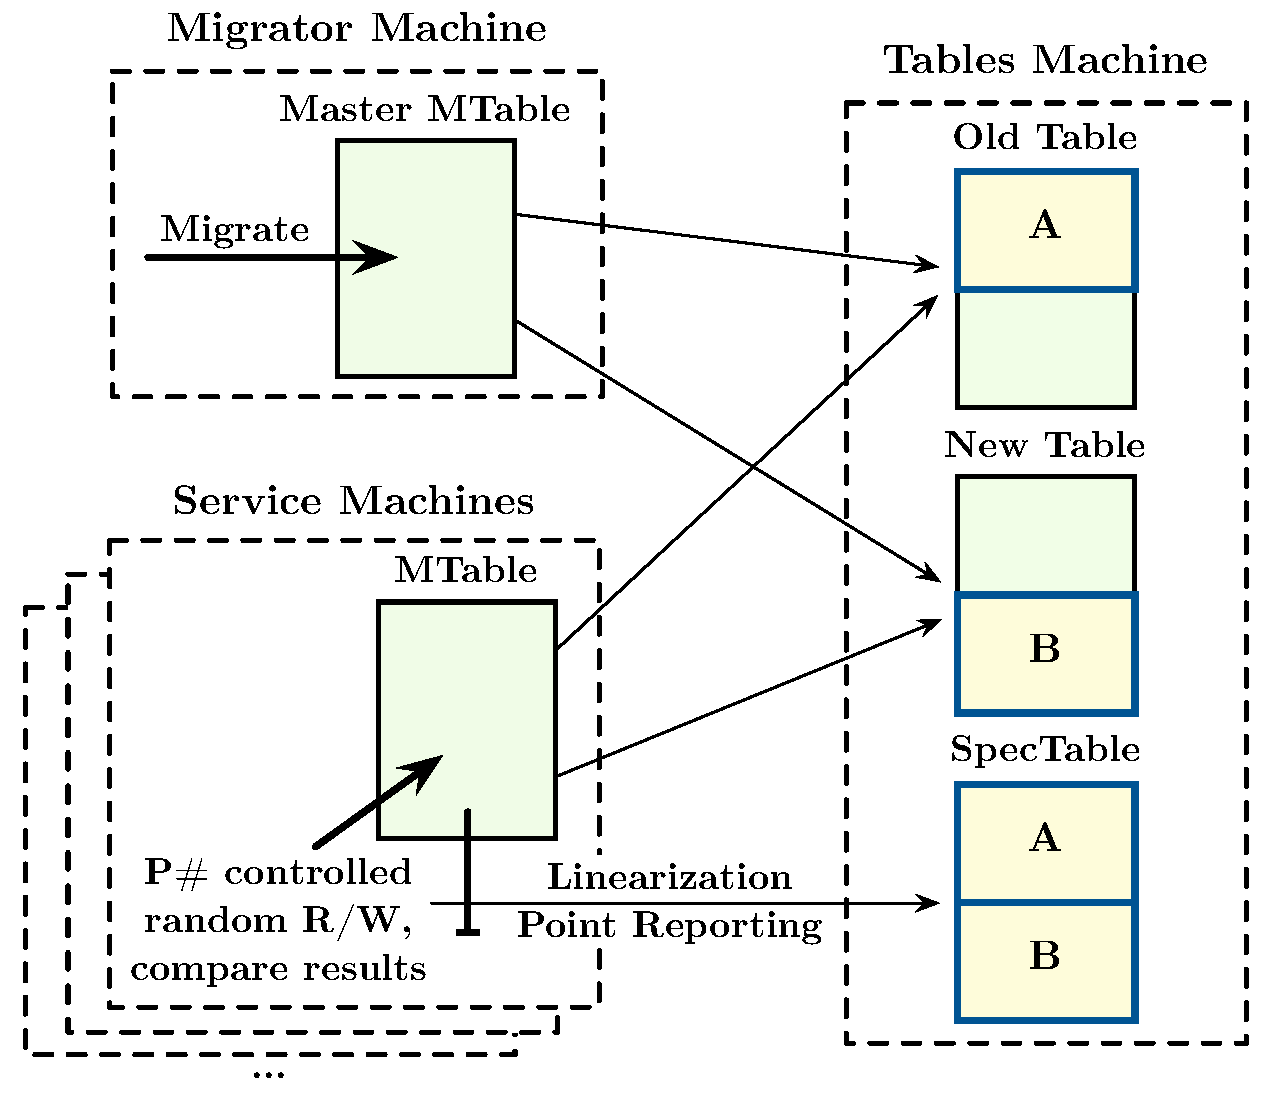
\includegraphics[width=\linewidth]{img/modeled_migration}
\vspace{-6mm}
\caption{The \psharp test environment of MigratingTable (each box with a dotted line represents one \psharp machine).}
\label{fig:mockedmigration}
\vspace{-2mm}
\end{figure}

The complete test environment is shown in Figure~\ref{fig:mockedmigration}. It consists of a \texttt{Tables} machine, which contains the BTs and RT, and serializes all operations on these tables; a set of \texttt{Service} machines that contain identically configured MTs; and a \texttt{Migrator} machine that performs the background migration. Each \texttt{Service} machine issues a random sequence of logical operations to its MT, which performs the backend operations on the BTs via \psharp events. The developers instrumented the MTs to report the \emph{linearization point} of each logical operation, i.e., the time at which it takes effect on the VT, so the test harness could perform the operation on the RT at the same time. (More precisely, after processing each backend operation, the \texttt{Tables} machine enters a \psharp state that blocks all further work until the MT reports whether the backend operation was the linearization point and, if so, the logical operation has been completed on the RT. This way, the rest of the system never observes the RT to be out of sync with the VT.)
% In my reading, the parentheses make it clear that we're amending the previous
% sentence; without them, it looks more like a contradiction. ~ Matt 2016-01-21
% Note: If the tables were observed to be out of sync, it could cause both false
% positives and false negatives. ~ Matt 2015-12-31
% Join paragraphs to save space
For further implementation details of MigratingTable and its test harness, we refer the reader to the source code repository~\cite{migratingtable-src}.

%\begin{figure}[t]
%\centering
%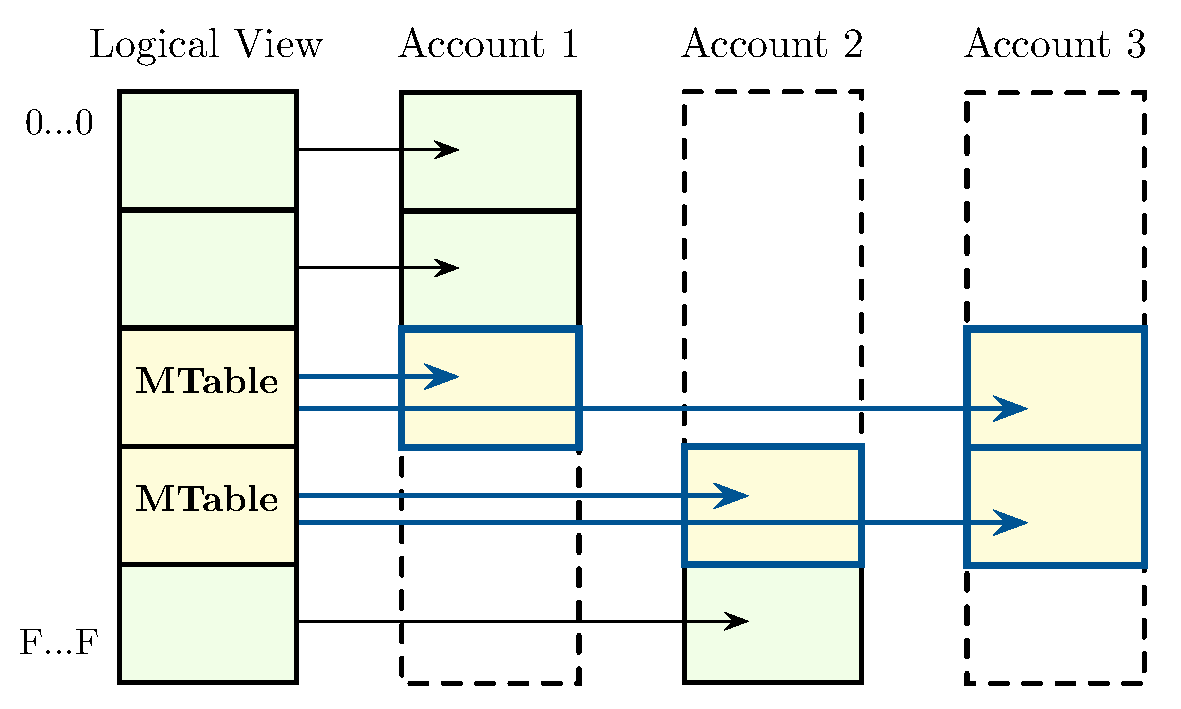
\includegraphics[width=\linewidth]{img/livemigration}
%\caption{Resharding a data set when a third Azure storage account is added. Two key ranges are each migrated to the new account using a MigratingTable instance (abbreviated MTable).}
%\label{fig:livemigration}
%\end{figure}

% N.B. Artifact Services is mentioned at http://research.microsoft.com/en-us/people/schulte/.  Hopefully it's OK to reveal that it was the system in this case study. ~ Matt 2015-08-17
%The initial motivation for MigratingTable was to solve a scaling problem for Artifact Services, an internal Microsoft system with a data set that is sharded across tables in different Azure storage accounts because it exceeds the limit on traffic supported by a single Azure storage account.  As the traffic continues to grow over time, the system needs to reshard the data set across a greater number of Azure storage accounts without interrupting service.  During such a resharding, our sharding manager will identify each key range that should migrate to a different table, and we will use a separate MigratingTable instance for each such key range to actually perform the migration (Figure~\ref{fig:livemigration}).  MigratingTable may also be useful to migrate data to a table with different values of configuration parameters that Azure does not support changing on an existing table, such as geographic location.

%Since we were designing a new concurrent protocol that we expected to become increasingly complex over time as we add optimizations, we planned from the beginning to maintain a \psharp test harness along with the protocol to maintain confidence in its correctness.

%MigratingTable implements an interface called \texttt{IChainTable}, which provides the core read and write functionality of the original Azure table API with one exception: it provides \emph{streaming reads} with a weaker consistency property than multi-page reads in the original API, since the original property would have been difficult to achieve for no benefit to applications we could foresee.  MigratingTable requires that its backend tables also implement \texttt{IChainTable}, and we wrote a simple adapter to expose physical Azure tables as \texttt{IChainTable}.

% N.B. \texttt{SpecTable} = InMemoryTableWithHistory in the current codebase. ~ Matt 2015-08-17

%\psharp takes control of the choice of input history, as well as the schedule, so both can be reproduced using a single random seed. Then, under the \emph{small scope hypothesis} that any bug in MigratingTable leads to incorrect output for at least one input history in our distribution, we have a positive probability of detecting this incorrect output on each \PTComment{execution [iteration]} of the \psharp test.

%If we had no formalization of the specification and had to rely on expected outputs worked out by hand, this might be the best we could do.  However, since the \texttt{IChainTable} specification is relatively simple and is almost deterministic under sequential calls, it was straightforward to write an in-memory reference implementation called \texttt{SpecTable} to which we can compare the output of MigratingTable on an arbitrary input history.  This gave us the attractive option to sample from a distribution we defined over all possible input histories within certain bounds.

%It was convenient to let \psharp control the choice of input history as well as the schedule so we could reproduce both using a single random seed.  Then, under the \emph{small scope hypothesis} that any bug in MigratingTable leads to incorrect output for at least one input history in our distribution, we have a positive probability of detecting this incorrect output on each \PTComment{execution [iteration]} of the \psharp test.

%All of our input histories include two application processes.  Each process performs either a single streaming read or a sequence of two atomic calls, each a read or a batch write.  Each batch write call includes one or two operations, where the operation type is chosen from the set supported by \texttt{IChainTable} (Insert, Replace, Merge, Delete, InsertOrReplace, InsertOrMerge, DeleteIfExists) and the row key is chosen from $\{0, \ldots, 5\}$.  If the operation requires an If-Match value, it is equally likely to be \texttt{*}, the current ETag of the row (if it exists), or some non-matching value.  Finally, the new entity includes a user-defined property \texttt{isHappy} whose value is equally likely to be true or false.  For both atomic and streaming reads, the filter expression is equally likely to be empty (i.e., match everything), \texttt{isHappy eq true}, or \texttt{isHappy eq false}.

%As mentioned above, the \texttt{IChainTable} specification is almost deterministic under sequential calls; the only nondeterminism is in the results of streaming reads.  Given a streaming read, \texttt{SpecTable} can compute the set of all results that are compliant with the specification, so we can simply check if the result of MigratingTable is in this set.

%To test MigratingTable, we must supply it with backing tables.  We use \texttt{SpecTable} for this purpose as well, with \psharp choosing the actual result of each streaming read from the valid set.  Our correctness property is then:
% Convert to some theorem-like environment? ~ Matt
%\begin{quote}
%For every execution trace of a collection of MigratingTables backed by the same pair of \emph{old} and \emph{new} \texttt{SpecTable}s in parallel with the migrator job, there exists a linearization of the combined input history such that the output in the original trace matches the output of a ``reference'' \texttt{SpecTable} on the linearized input.
%\end{quote}
%

%The MigratingTable was instrumented to report the intended \emph{linearization point} of each input call, which in our setting is always one of the corresponding \emph{backend calls} to the backend tables (often the last).  Specifically, after each backend call completes, MigratingTable reports whether that call was the linearization point, which may depend on the result of the call.  This makes it possible to check the correctness property as the model executes.

%We use the \psharp random scheduling strategy; we were afraid that an exhaustive strategy would only be feasible within bounds so low that we would miss some bugs.

%We wanted to implement the core MigratingTable algorithms in \csharp ``async/await'' code, like most of Artifact Services, to achieve both good readability and good performance.  We used a method similar to that described in \S\ref{sec:psharp:async} to bring the generated TPL tasks under the control of the \psharp scheduler.  Then we implemented an ``async'' RPC mechanism based on the .NET RealProxy class that automates the generation of proxies for objects hosted by other \psharp machines (in our setting, the service machines use proxies for the \texttt{SpecTable}s and various auxiliary objects hosted by the tables machine).  When a machine calls a method on a proxy, the proxy sends a \psharp message to the host machine, causing it to execute the method call on the original object and send back the result, which the proxy then returns.  Thus, the use of these proxies as \texttt{IChainTable} backends is transparent to the MigratingTable library, thanks to dynamic dispatch.
